\section{Results}
As it can be observed on Figures \ref{fig:case1}, \ref{fig:case2} and
\ref{fig:case3}, the different cascade levels required up to $2n+1$, with $n$ the
level number to start enriching uranium. This corresponds to the time required
for the material to propagate from the natural uranium source to the level,
regardless of the duration of the timestep (hour, day, month,...). This is also
true for the number of timestep required to reach the equilibrium assays value in
the tail reprocessing cases. This is why one will only consider equilibrium
values.

\begin{table}[h!]
\centering
  \caption{Summary of cascades level population.}
\begin{tabular}{ccccccccc}
\toprule

Model       &        &           & A         & A         & B         & B       & C         & C          \\
Recycling   &        &           & No        & yes       & No        & Yes     & No        & yes        \\
\midrule                                                                                                 
        &            & Feed      & $0.71w\%$ & $1.3w\%$  & $0.71w\%$ & $0.94w\%$ & $0.71w\%$ & $1.66w\%$ \\
Level 0 & Assay      & Product   & $4.13w\%$ & $7.7w\%$  & $4.13w\%$ & $5.43w\%$ & $4.13w\%$ & $9.53w\%$ \\
        &            & Tail      & $0.29w\%$ & $0.5w\%$  & $0.29w\%$ & $0.39w\%$ & $0.29w\%$ & $0.69w\%$  \\
        & Cascades   &           & 26.73     & 26.45     & 26.6      & 25.8      & 26.73     & 26.45      \\
\midrule                                                                                                 
        &            & Feed      & $4.13w\%$ & $11.9w\%$ & $4.13w\%$ & $6.84w\%$ & $4.13w\%$ & $13.0w\%$ \\
Level 1 & Assay      & Product   & $22.8w\%$ & $55.7w\%$ & $20.6w\%$ & $30.7w\%$ & $22.9w\%$ & $69.8w\%$ \\
        &            & Tail      & $1.8w\%$  & $6.6w\%$  & $1.72w\%$ & $2.91w\%$ & $1.81w\%$ & $9.43w\%$  \\
        & Cascades   &           & 2.92       & 3.20      & 2.91      & 3.41     & 2.92      & 3.20       \\
\midrule                                                                                                 
        &            & Feed      & $22.8w\%$ & $55.7w\%$ & $20.6w\%$ & $34.3w\%$ & $22.9w\%$ & $72.6w\%$ \\
Level 2 & Assay      & Product   & $78.5w\%$ & $95.0w\%$ & $61.0w\%$ & $75.8w\%$ & $82.0w\%$ & $98.4w\%$ \\
        &            & Tail      & $4.12w\%$ & $50.9w\%$ & $9.56w\%$ & $17.5w\%$ & $15.7w\%$ & $69.4w\%$ \\
        & Cascades   &           & 0.31      & 0.35      & 0.37      & 0.64      & 0.32      & 0.35      \\
\midrule                                                                                                 
        &            & Feed      & $78.5w\%$ & N.A.      & $61.0w\%$ & $75.8w\%$ & $82.3w\%$ & N.A.      \\
Level 3 & Assay      & Product   & $98.2w\%$ & N.A.      & $90.4w\%$ & $95.0w\%$ & $99.1w\%$ & N.A.      \\
        &            & Tail      & $76.1w\%$ & N.A.      & $79.3w\%$ & $56.1w\%$ & $80.3w\%$ & N.A.      \\
        & Cascades   &           & 0.03      & N.A.      & 0.080     & 0.18      & 0.03      & N.A.      \\
\bottomrule
\end{tabular}
  \label{tab:level}
\end{table}


\begin{figure}[h!]
    \centering
    \begin{subfigure}[t]{0.45\textwidth}
        \centering
        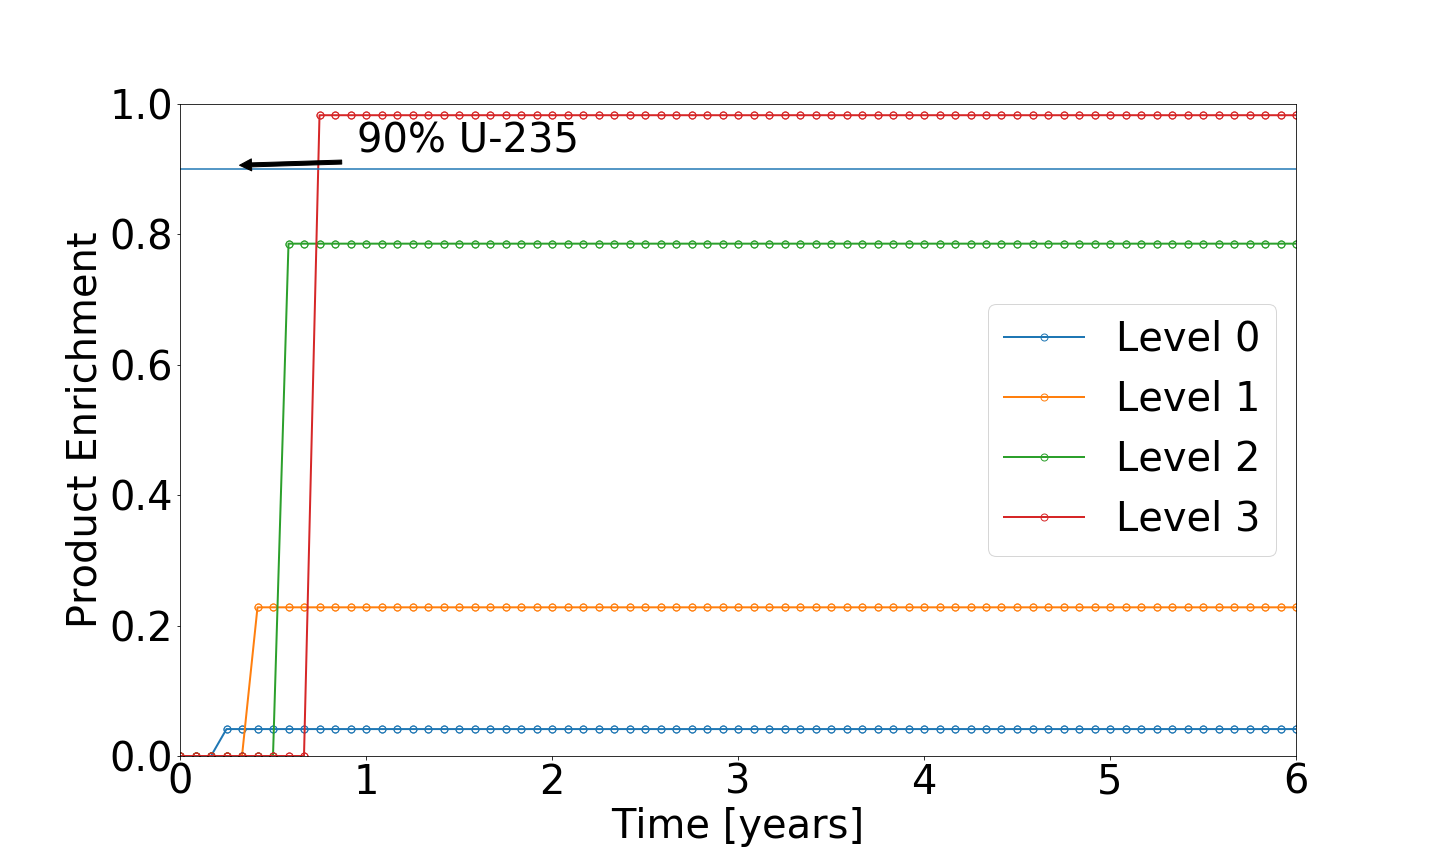
\includegraphics[scale=0.18]{NR_case1}
        \caption{No tail recycling}
        \label{sfig:case1_NR}
    \end{subfigure}%
    \begin{subfigure}[t]{0.45\textwidth}
        \centering
        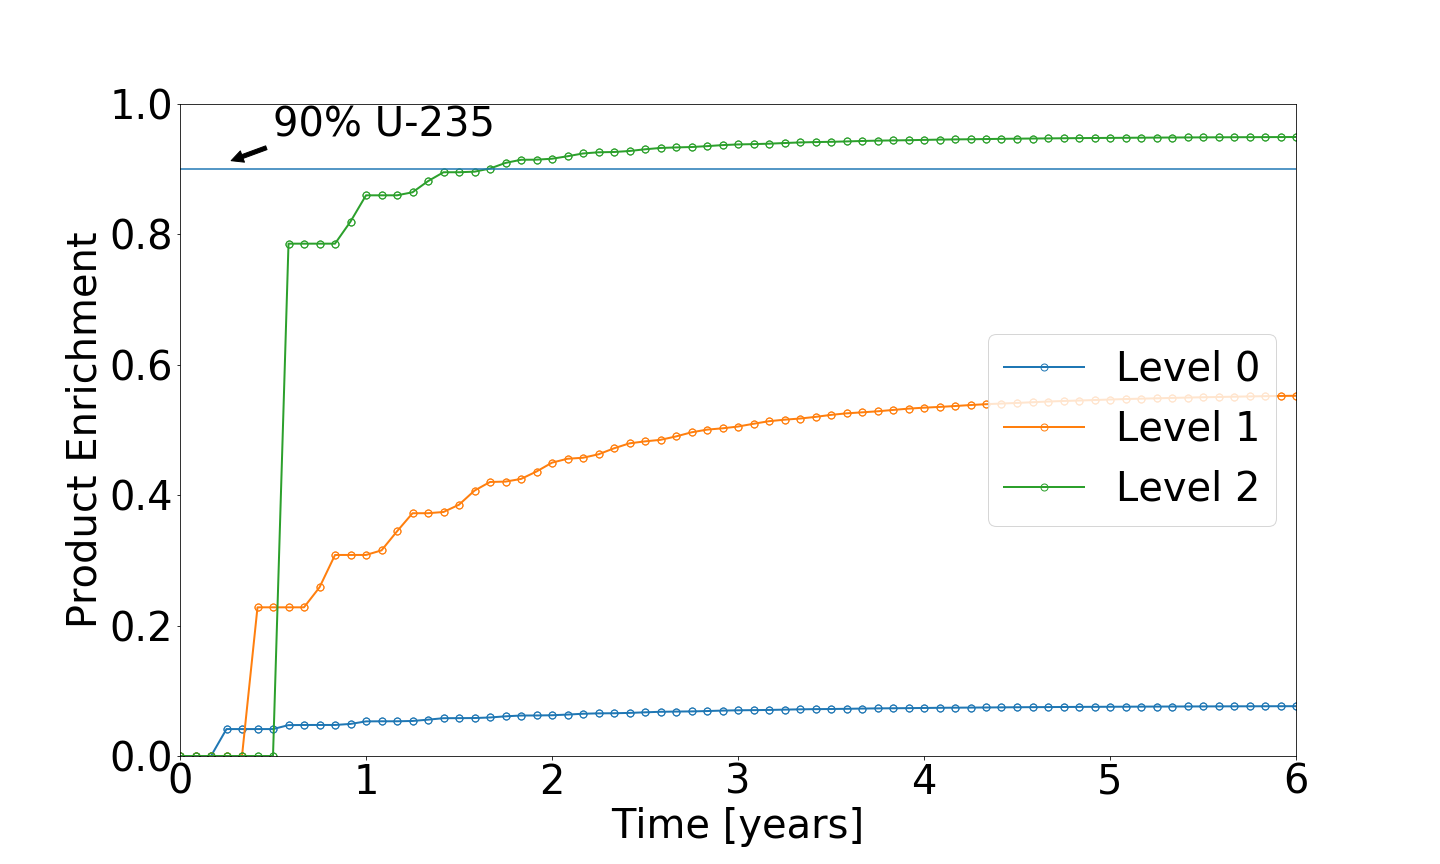
\includegraphics[scale=0.18]{R_case1}
        \caption{Tail recycling}
        \label{sfig:case1_R}
    \end{subfigure}
    \caption{Evolution of the product assays at each level with considering
    miss-use model A, with (right) and without recycling (left).}
    \label{fig:case1}
\end{figure}

\subsection{Miss-use modeling}
As illustrated on Figures \ref{sfig:case1_NR}, \ref{sfig:case2_NR} and
\ref{sfig:case3_NR} and summarized on Tab \ref{tab:level}, the different model
don't have the same effect on the cascade behavior. While the models A and C,
allow a quick enrichment gain, when the chaining the enrichment cascades, respectively
4/23/78/98 and 4/23/82/99, with model B, the enrichment gain is slower only
4/21/61/90...
The same effect is observed when recycling the tails\ldots

\begin{figure}[h!]
    \centering
    \begin{subfigure}[t]{0.45\textwidth}
        \centering
        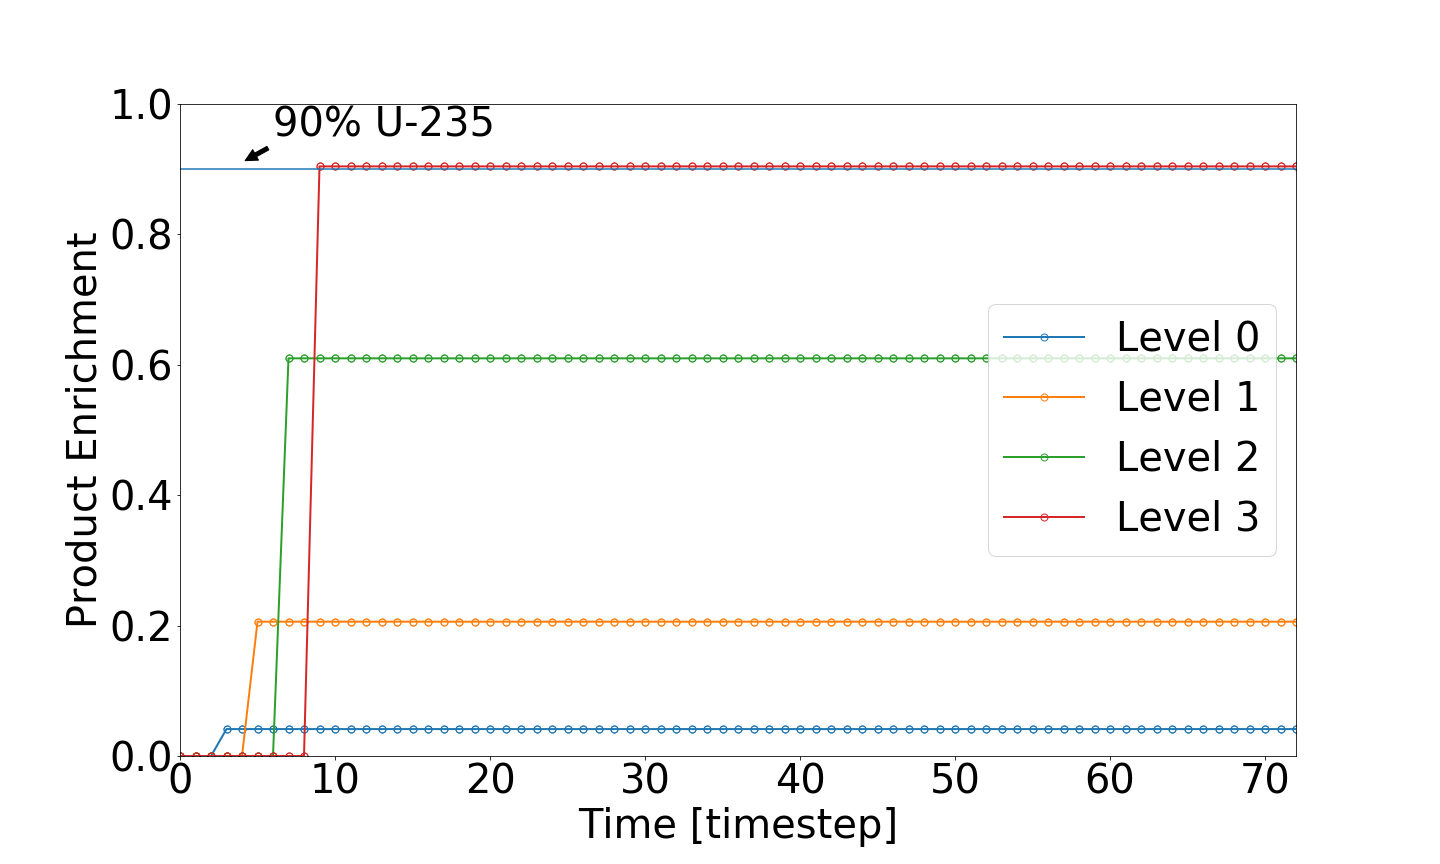
\includegraphics[scale=0.18]{NR_case2}
        \caption{No tail recycling}
        \label{sfig:case2_NR}
    \end{subfigure}%
    \begin{subfigure}[t]{0.45\textwidth}
        \centering
        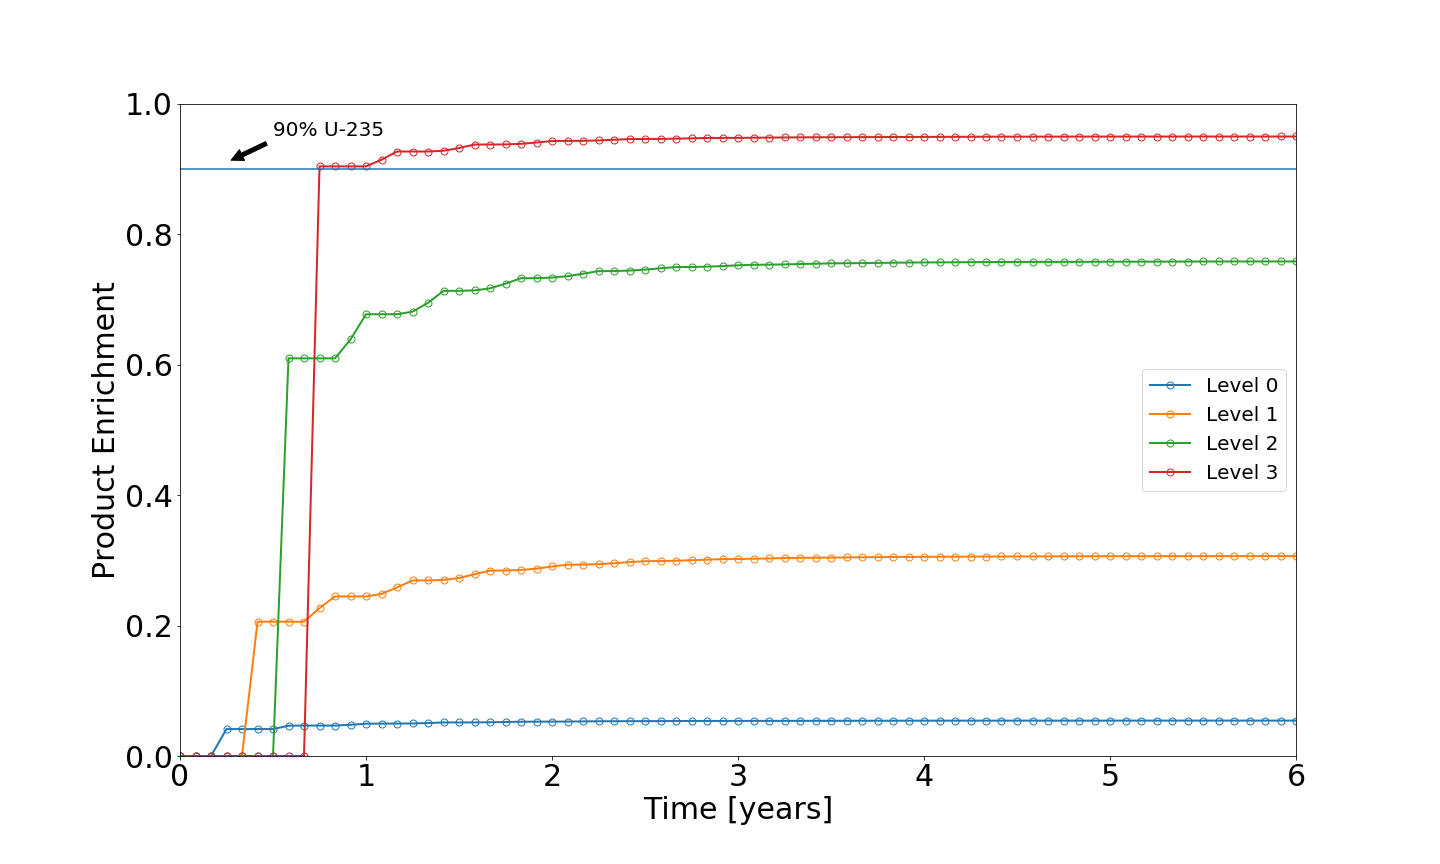
\includegraphics[scale=0.18]{R_case2}
        \caption{Tail recycling}
        \label{sfig:case2_R}
    \end{subfigure}
    \caption{Evolution of the product assays at each level with considering
    miss-use model B, with (right) and without recycling (left).}
    \label{fig:case2}
\end{figure}

\subsection{Tails recycling}
As demonstrated on Figures \ref{sfig:case1_R}, \ref{sfig:case2_R} and
\ref{sfig:case3_R}, recycling the tails increases the overall product assay at all
the different levels. As shown on Table \ref{tab:level}, the tail assay of level
$n$ is always higher than the product assay of level $n-2$, recycling the tails
of level $n$ will consequently increase the feed assay of level $n-1$. Moreover,
as the feed assay of level $n-1$ increases, its tail and product assays increase as well,
increasing de facto the feed assays of respectively cascade levels $n-2$ and $n$...
This effect allow to reduce the number of cascade levels required to reach
\gls{HEU} in case A and C.

\begin{figure}[h!]
    \centering
    \begin{subfigure}[t]{0.45\textwidth}
        \centering
        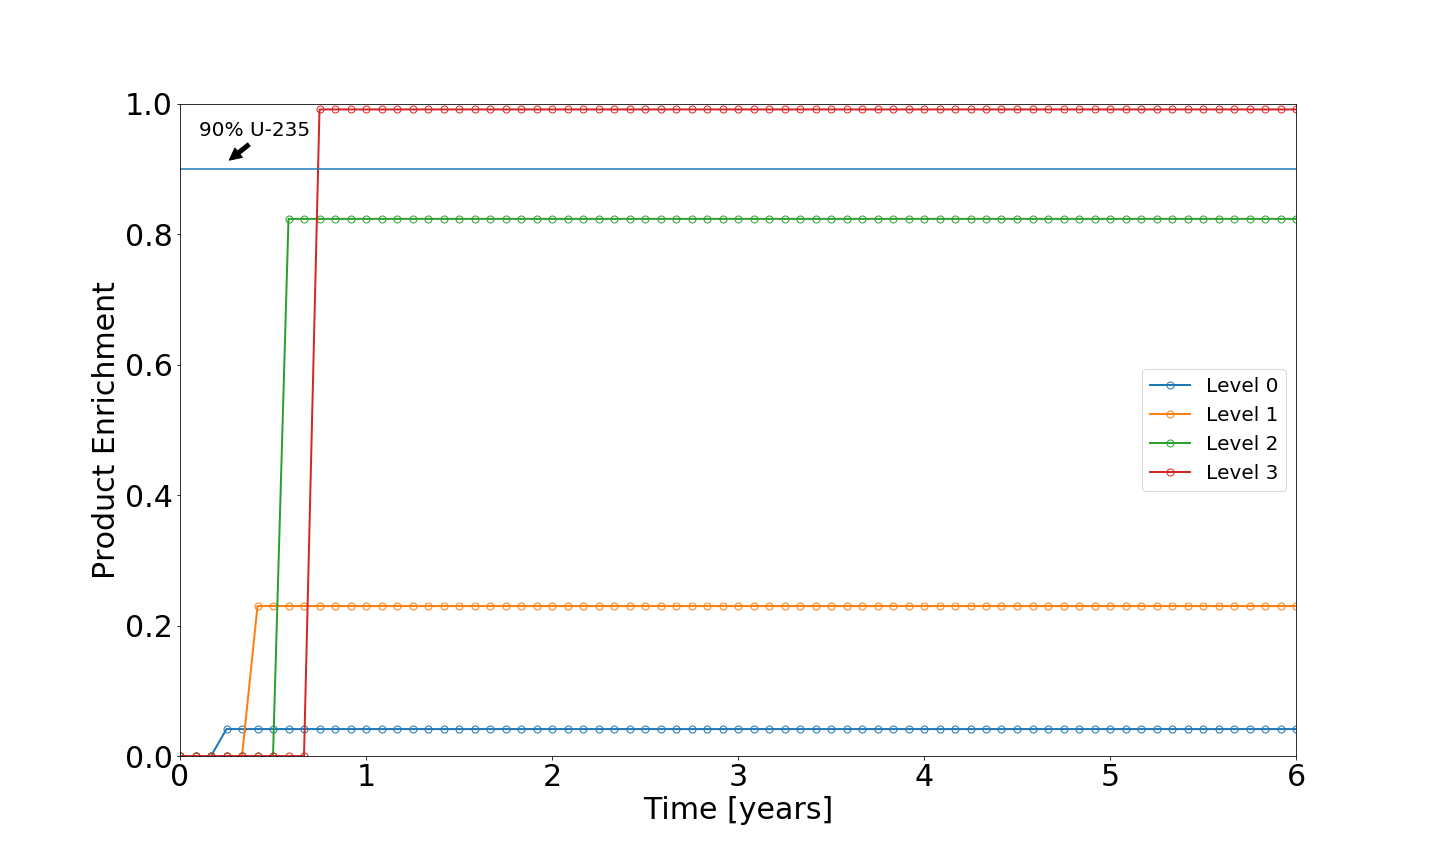
\includegraphics[scale=0.18]{NR_case3}
        \caption{No tail recycling}
        \label{sfig:case3_NR}
    \end{subfigure}%
    \begin{subfigure}[t]{0.45\textwidth}
        \centering
        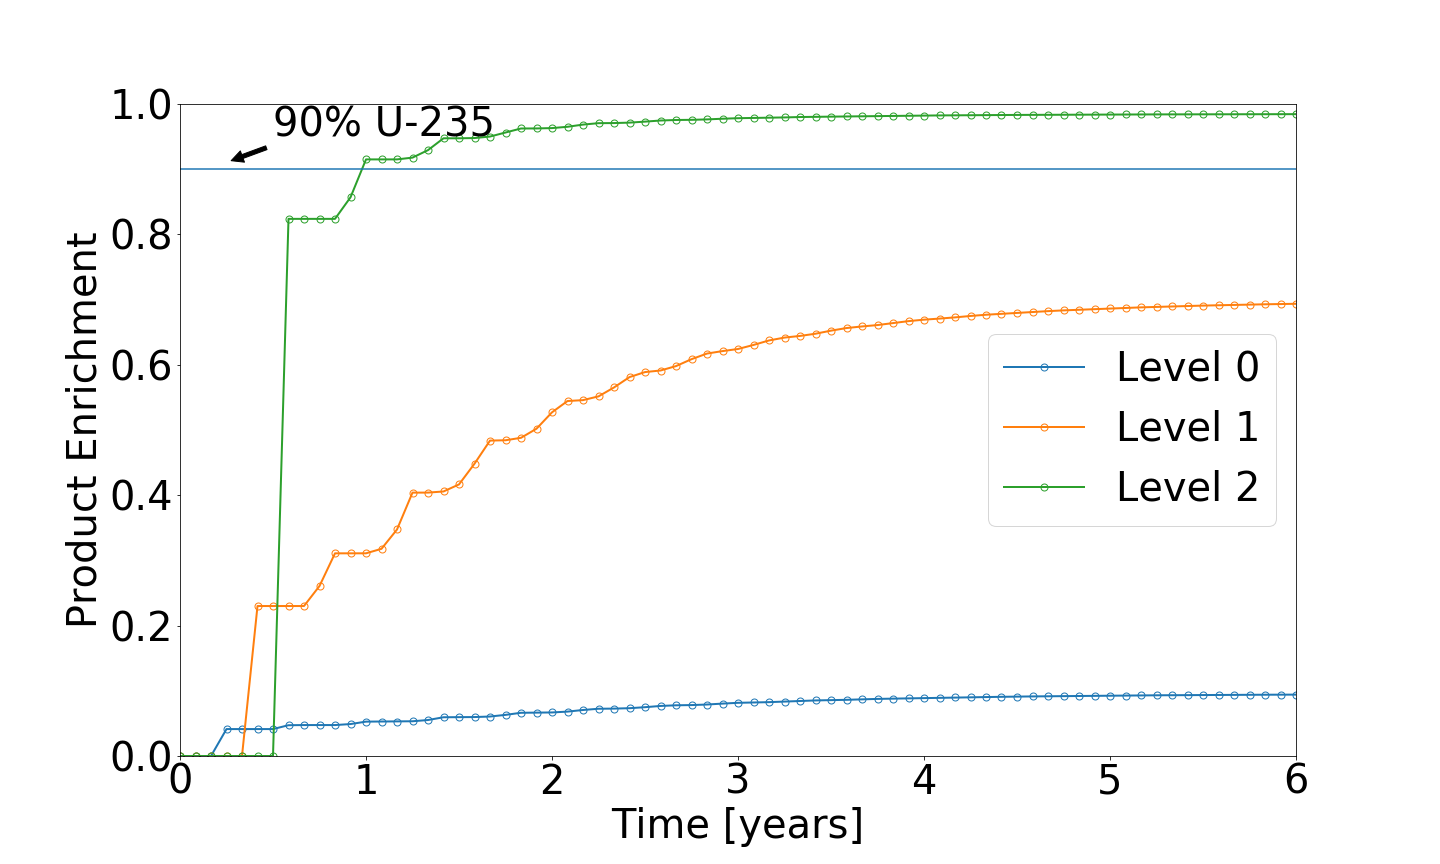
\includegraphics[scale=0.18]{R_case3}
        \caption{Tail recycling}
        \label{sfig:case3_R}
    \end{subfigure}
    \caption{Evolution of the product assays at each level with considering
    miss-use model C, with (right) and without recycling (left).}
    \label{fig:case3}
\end{figure}



\subsection{Production}

\begin{figure}[h!] % replace 't' with 'b' to force it to be on the bottom
    \centering
    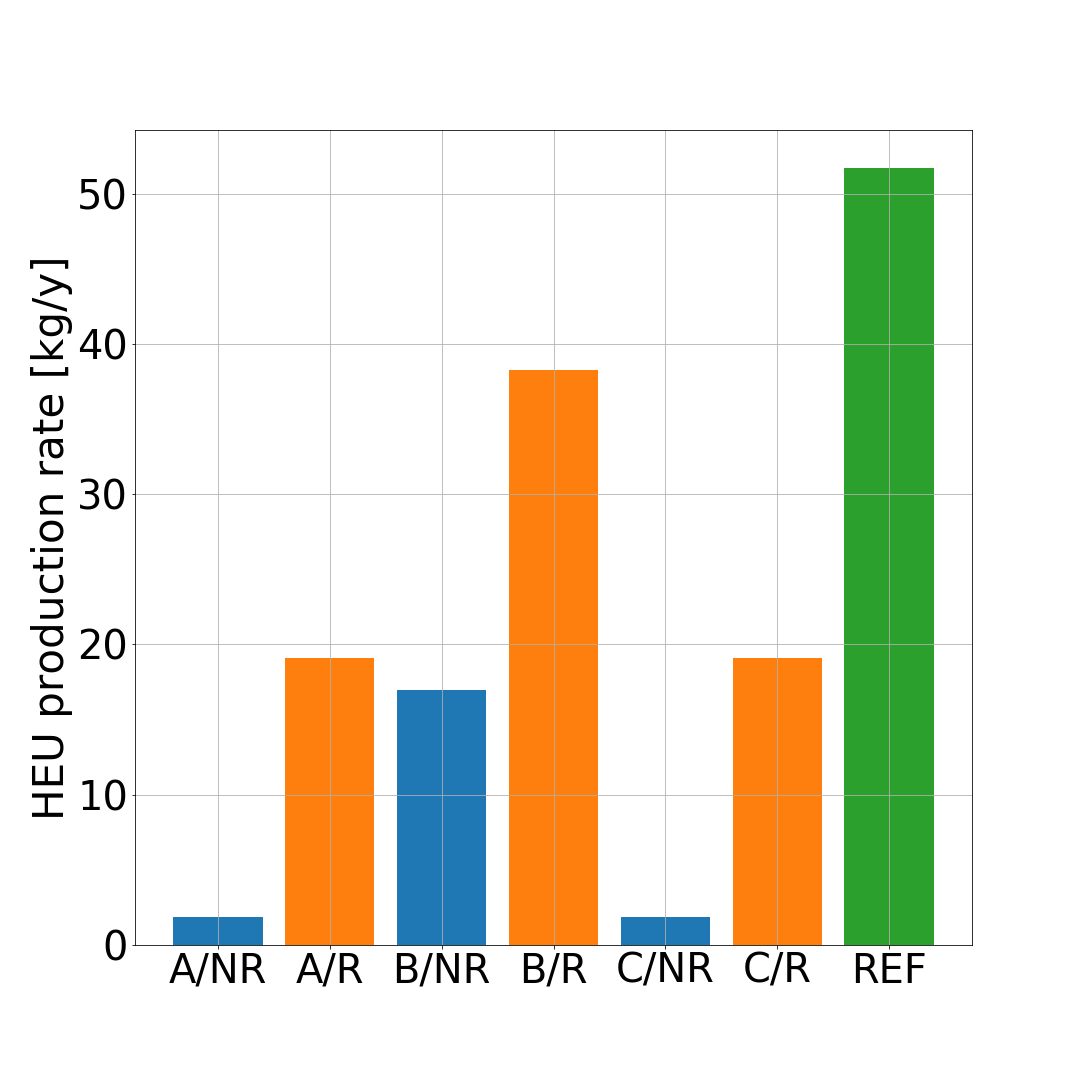
\includegraphics[scale=0.25]{HEU_prod_rate}
    \caption{Production rate for the different model configuration, with in blue
    the case without tail recycling, in orange with tail recycling, and in green
    the reference one. Where A-B-C represent the model used, and NR-R
    respectively the case without tail recycling and the case with tail recycling}
    \label{fig:HEU_rate}
\end{figure}
